Po niej \textbf{przyszedł na świat 5 czerwca 1913 r. w Łagiewnikach Wielkich Wiktor Świerczyński}.

\begin{figure}[!h]
\begin{center}
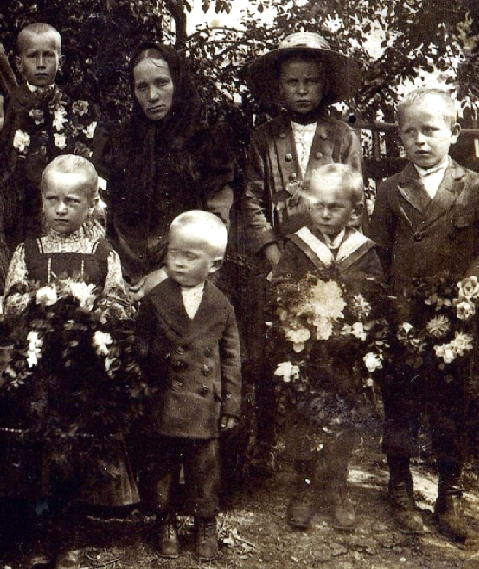
\includegraphics[width=0.4\textwidth]{photo/wiktor_swierczynski_1.jpg}
\caption[Wiktor Świerczyński z mamą Eufemią]{Wiktor Świerczyński stoi najmniejszy w marynarce przed swoją mamą Eufemią (fragment zdj. z pogrzebu pradziadka Jakuba Grabińskiego).}
\label{rys:wiktor_swierczynski_1}
\end{center}
\end{figure}

Przeszedł on w wieku szkolnym, gdzieś około 14 roku życia zapalenie opon mózgowych, co w wyniku powikłań było przyczyną niedowładu nóg. Mógł się poruszać czołgając się lub jeżdżąc na skonstruowanym przez siebie wózku inwalidzkim. Był bowiem bardzo zdolnym młodzieńcem! Jego młodszy brat Benedykt tak o nim wspomina: \textit{Wiktor, to pechowiec, którego dopadł wirus Heinego – Mediny (wtedy jeszcze nieznany) – jak on się męczył tygodniami i został kaleką (porażenie kończyn dolnych i zwyrodnienie kręgosłupa), nie mówiąc już o tym jak on się czuł wśród zdrowych}.

\begin{figure}[!h]
\begin{center}
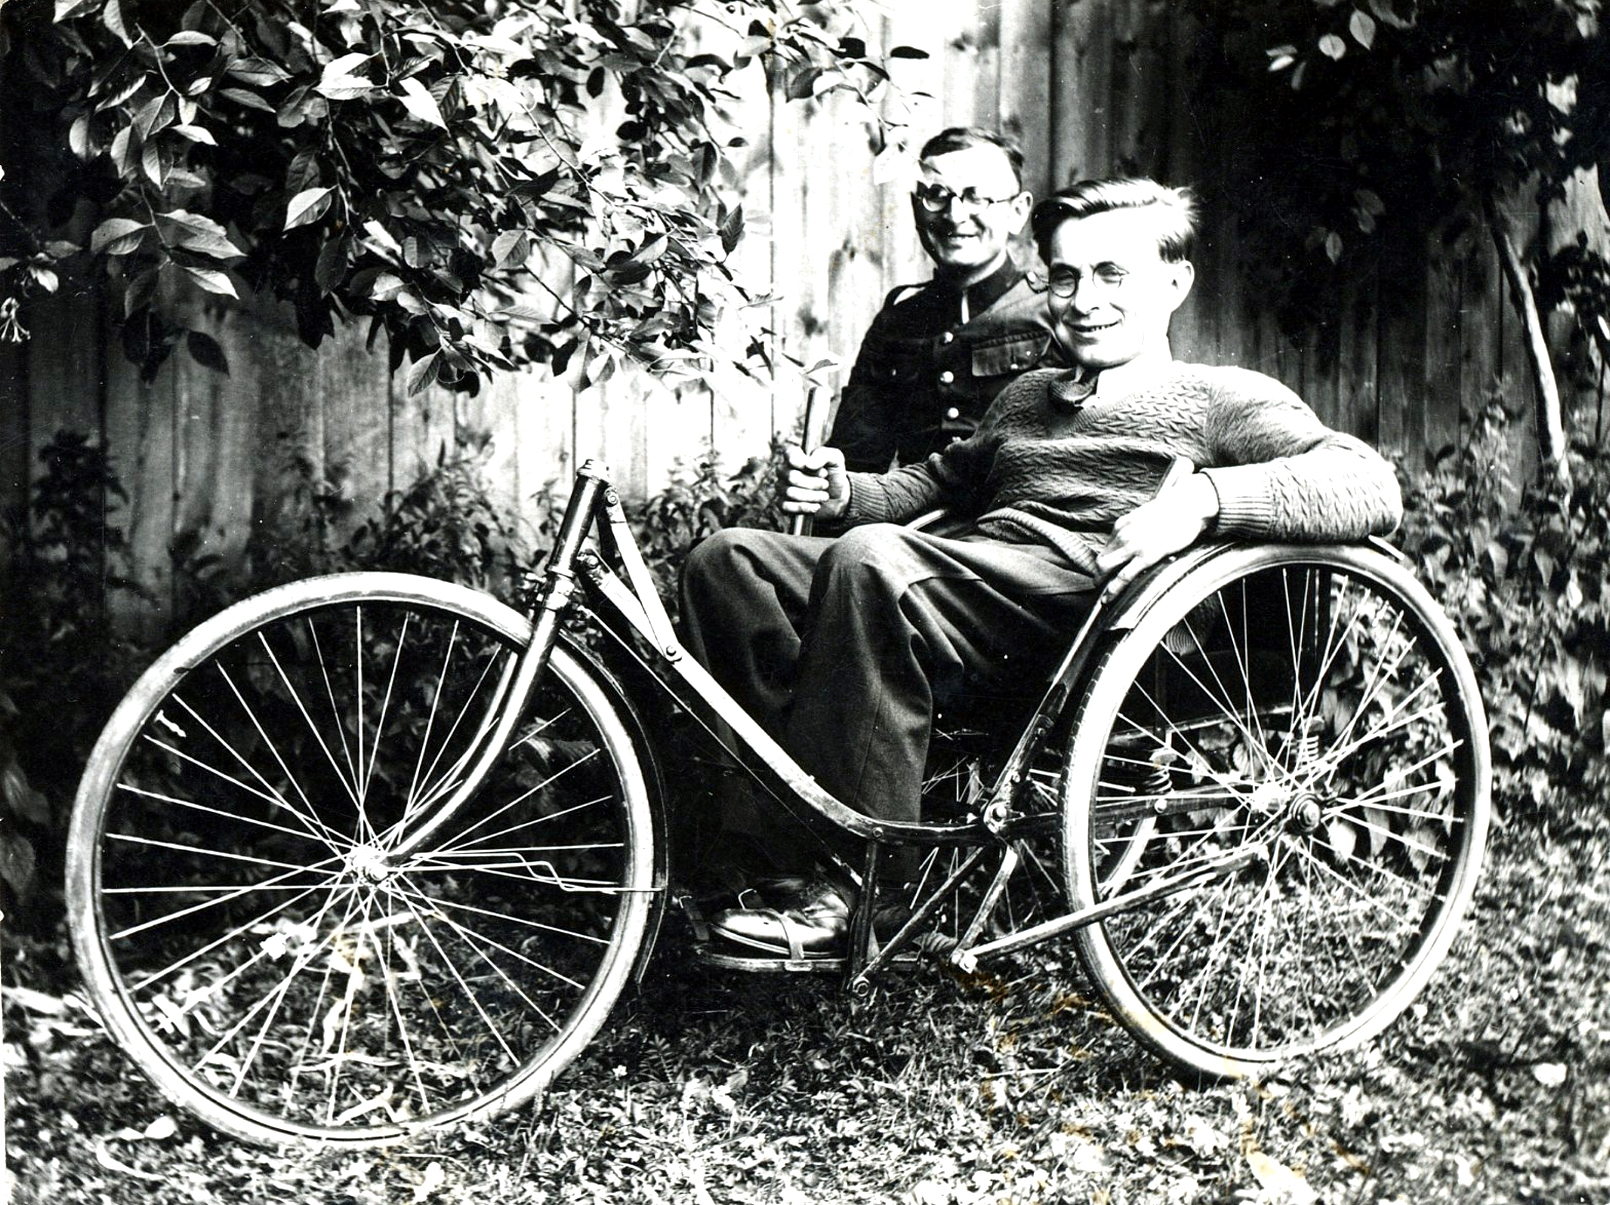
\includegraphics[width=0.7\textwidth]{photo/wiktor_swierczynski_2.jpg}
\caption[Wiktor Świerczyński i Antoni Lehman]{Wiktor Świerczyński na wózku inwalidzkim przez siebie skonstruowanym, za nim siedzi jego szwagier - Antoni Lehman.}
\label{rys:wiktor_swierczynski_2}
\end{center}
\end{figure}

Budował w tamtych czasach radia kryształkowe, naprawiał zegary, strugał dzieciom fujarki z kruszyny. Dzięki temu był samowystarczalny finansowo, nie będąc ciężarem dla licznej rodziny. Wszędzie był przyjmowany, a dzieci chętnie pomagały mu wjechać na górkę w Wieskach. Do kościoła był wnoszony jak dziecko -- na rękach, mimo to Mszy św. niedzielnej nie opuszczał, wbrew jakby upokarzającej świadomości, że jego rówieśnicy oglądają się już za pannami\ldots

\begin{figure}[!h]
\begin{center}
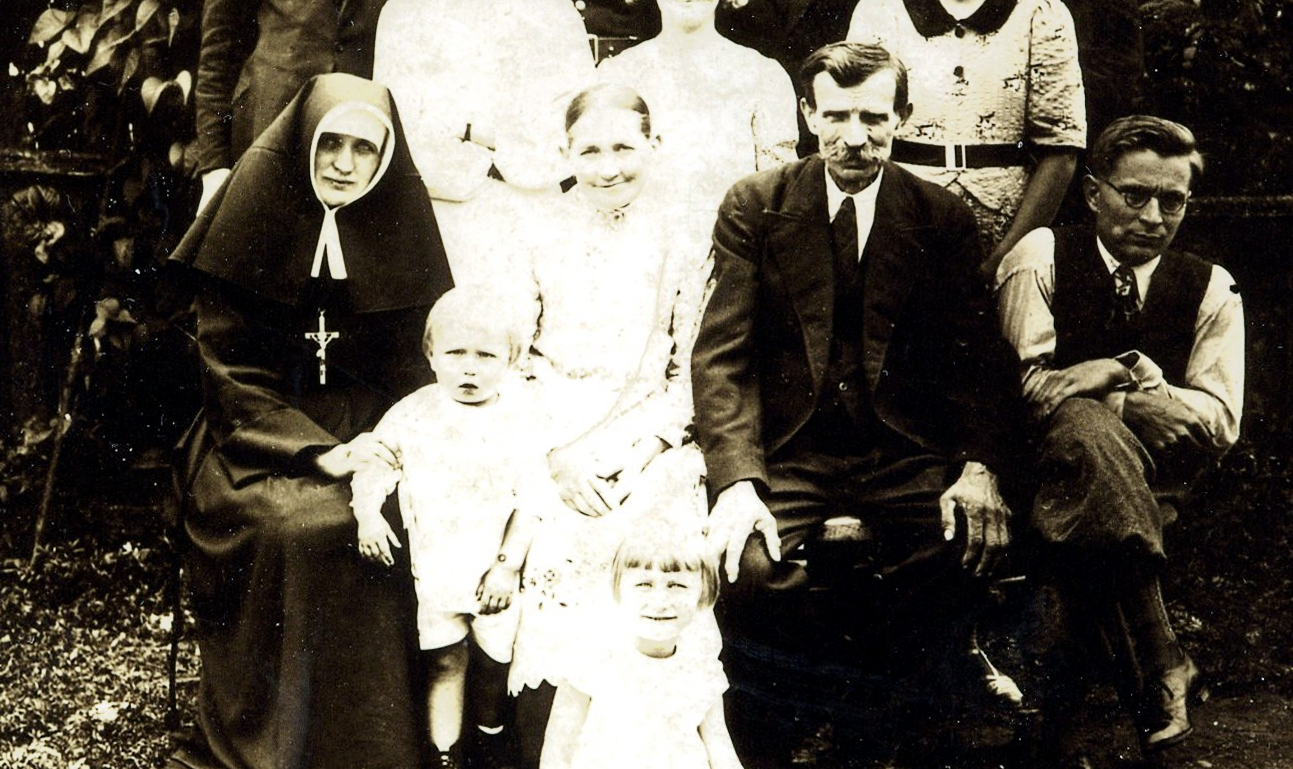
\includegraphics[width=0.7\textwidth]{photo/wiktor_swierczynski_3.jpg}
\caption[Wiktor Świerczyński z dziadkiem Edwardem]{Na zdj. Wiktor Świerczyński (siedzi po prawej obok dziadka Edwarda)}
\label{rys:wiktor_swierczynski_3}
\end{center}
\end{figure}

Gdy więc wuj Edward Grabiński zwany od swego zawodu Piekarzem (brat naszej babki Eufemii) zaproponował mu wyleczenie tego, co tak go upokarzało, chwycił się tej szansy z wielką nadzieją. Nie wiedział jednak ani on ani wujek Edward, że w Krüppelheimach pod hitlerowską władzą nie leczy się ludzi dotkniętych kalectwem, lecz traktuje się ich jak króliki doświadczalne, a w końcu się ich uśmierca!!! (hitlerowska eutanazja nic ludzkości nie nauczyła, skoro w Holandii i Belgii została wprowadzona jako ustawowy obowiązek lekarzy i szpitalnictwa -- oto jak unijne ustawodawstwo dorównało już poziomem hitlerowskiemu!!!). 

W Bytomskim Krüppelheimie (,,Domu Kalek'') stryjowi Wiktorowi niemieccy mordercy w lekarskich kitlach usztywnili nogi tak, że nie mógł już nawet siedzieć, a więc poruszać się na wózku inwalidzkim… Bardzo sobie wziął on do serca i głowy to tragiczne pogorszenie swojej sytuacji. Mawiał, że dotąd mógł się poruszać jak zwierzę, tzn. czołgając się, a teraz to z nim zrobili, że może leżeć jak kłoda, zawada, bo już nic dobrego nie może zmajstrować. W tej depresyjnej sytuacji Krüppelheim w Bytomiu przewiózł stryja Wiktora do Szpitala Psychiatrycznego w Lublińcu, by tam go mogli hitlerowcy w białych fartuchach bezkarnie uśmiercić!

\begin{figure}[!h]
\begin{center}
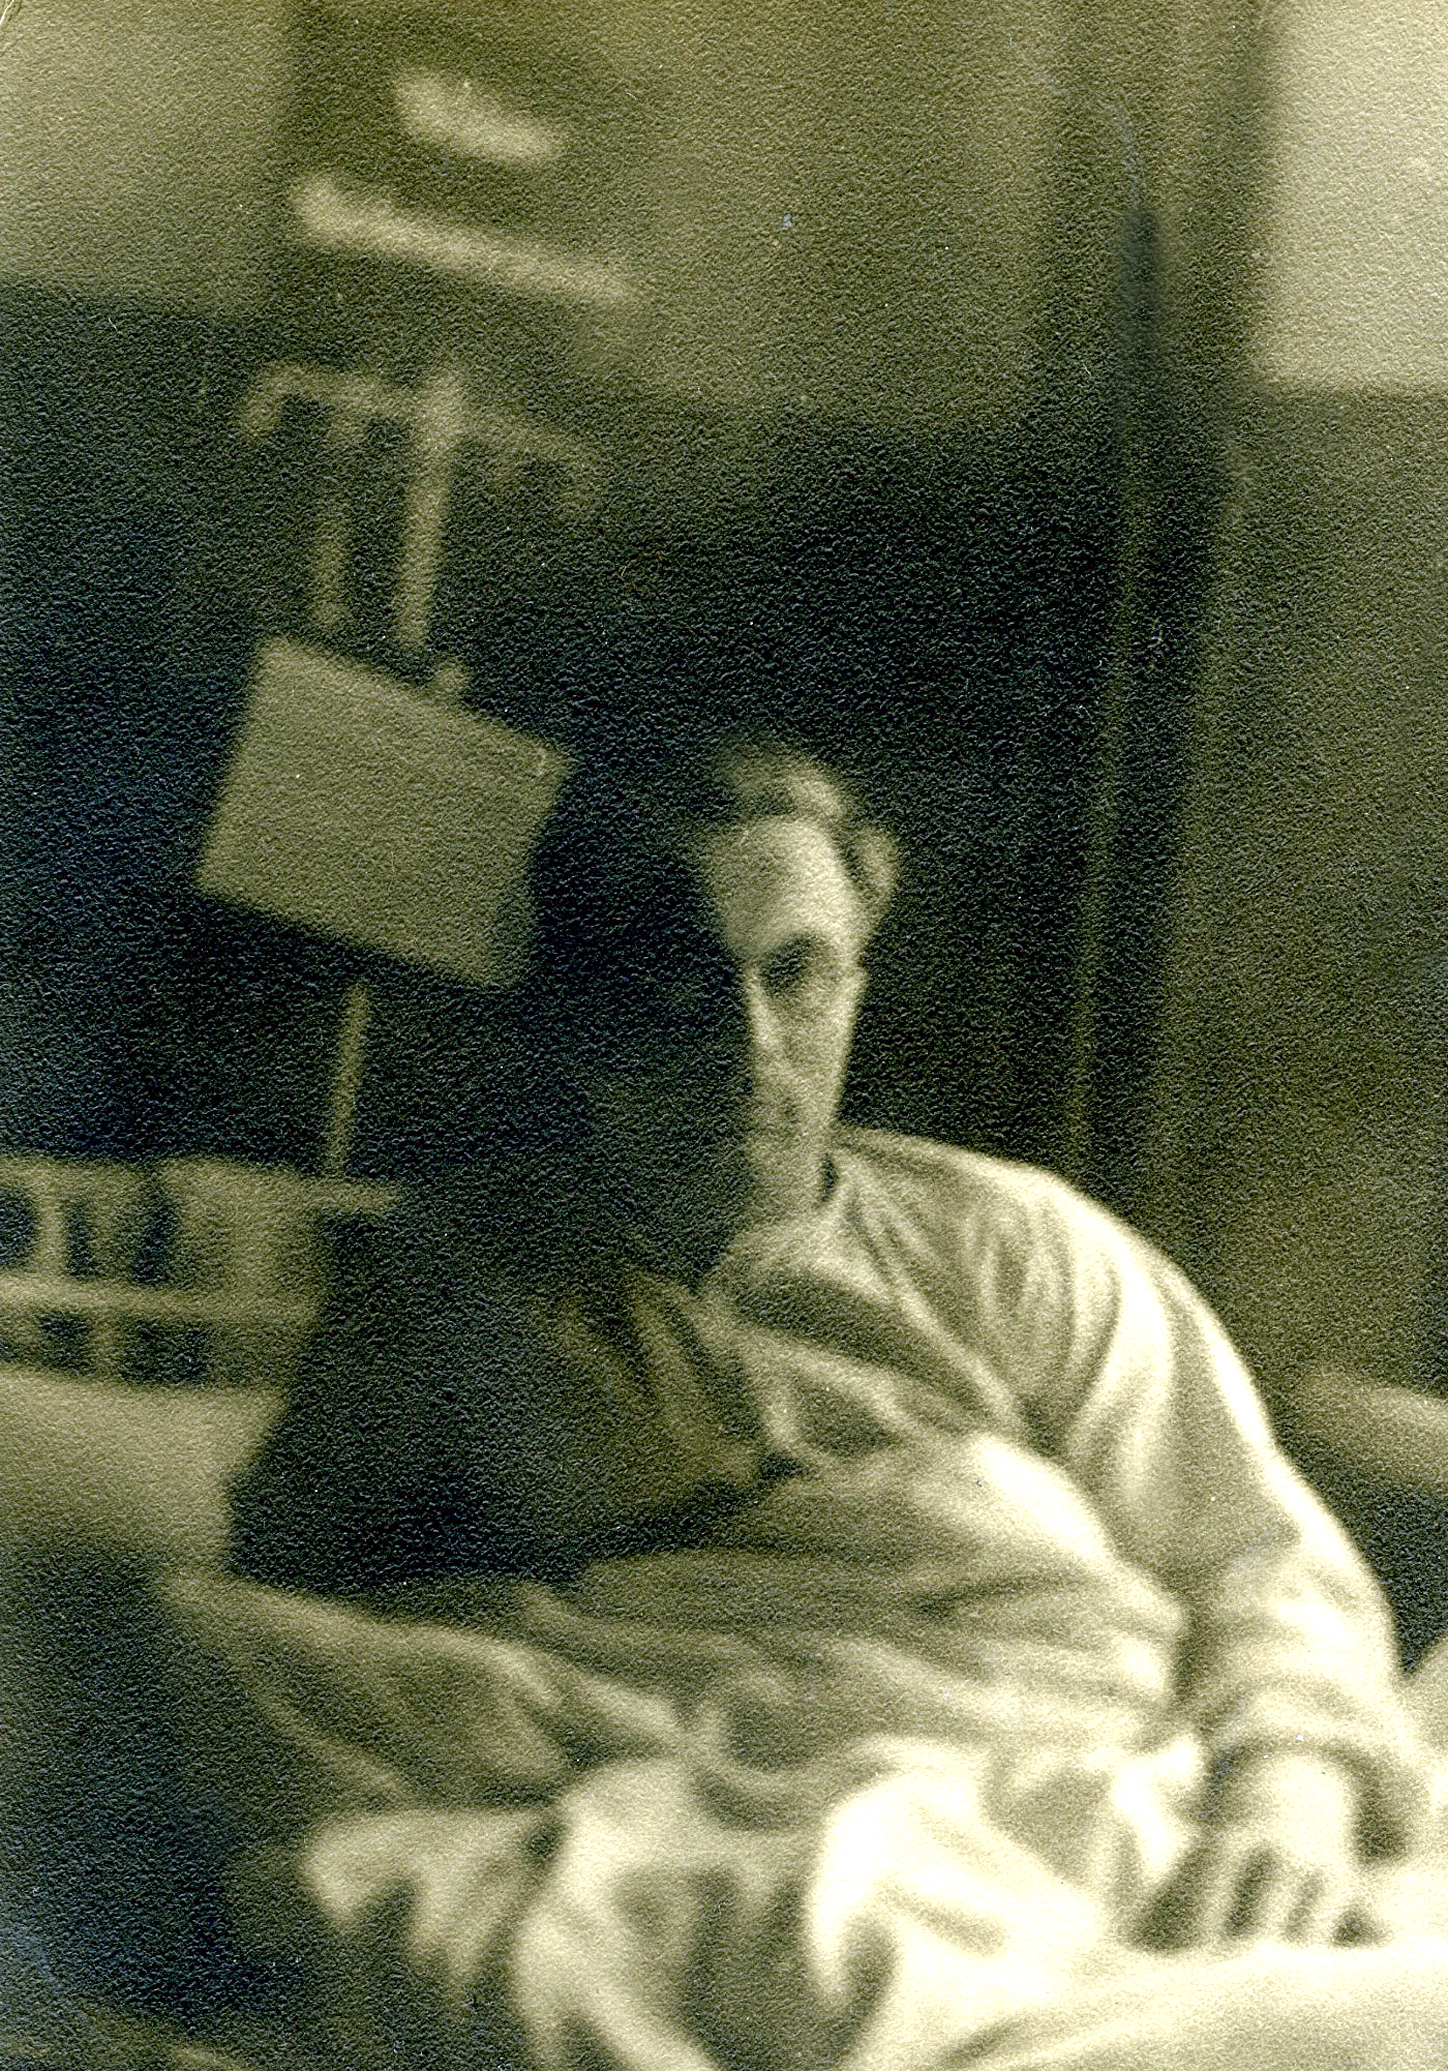
\includegraphics[width=0.35\textwidth]{photo/wiktor_swierczynski_4.jpg}
\caption{Wiktor Świerczyński w szpitalu}
\label{rys:wiktor_swierczynski_4}
\end{center}
\end{figure}

Miał on tę łaskę od Boga, że odwiedzili go w szpitalu wszyscy jego bliscy, szczególnie jego dwaj żyjący bracia, którzy służyli wtedy w wojsku niemieckim, jako obywatele III Rzeszy. Józef na zachodzie, w Magdeburgu, a Benedykt na froncie wschodnim, skąd nie można było otrzymać przepustki nawet na pogrzeb rodziców, ale dla Opatrzności Bożej nie ma nic niemożliwego, więc nasz tato – Benedykt otrzymał 11 maja 1942 r. ranę postrzałową od wybuchu granatu, w związku z czym dostał się do szpitala wojskowego w Dniepropietrowsku, a stamtąd na dłuższe leczenie i rehabilitację został przewieziony do szpitala w Traben -- Trarbach nad Mozelą (zachodnia strona Nadrenii, niedaleko Koblencji), a po wyleczeniu, dostał dwa tygodnie urlopu, więc przybył zaraz w rodzinne strony. Odwiedził od razu brata Wiktora, który leżał jak żywy trup i z wielką trudnością mówił -- widocznie podawali mu silne środki psychotropowe. Gdy przyjechał do niego brat Józef i interweniował w jego sprawie, bo znał świetnie urzędowy niemiecki, pseudolekarze ze swastyką w klapie wpadli w popłoch i postanowili stryja Wiktora niezwłocznie zamordować. Czuł on, co chcą z nim zrobić lub otrzymał od kogoś z personelu ostrzeżenie. Podzielił się tymi obawami z siostrą Anastazją (już wtedy siostrą zakonną Aurelią) i błagał ją, by go stamtąd zabrała, gdyż oni mają zamiar go wykończyć. Wtedy nie było taksówek, a ponadto stryj Wiktor miał sztywne nogi, więc można go było wynieść stamtąd tylko na noszach.\ldots

Gdy następnego dnia czerwcowego, dokładnie 24 czerwca 1942 r., w dzień narodzin św. Jana furmanką przyjechali po niego dziadek Edward z Edwardem Grabińskim ,,Piekarzem'', już stryj Wiktor nie żył, ponieważ, jak oficjalnie stwierdzili lekarze mordercy -- popełnił samobójstwo, wbijając sobie lufkę od papierosa w samo serce. Takie bajki nawet dzieciom nie godzi się opowiadać, gdyż na kilometr cuchną oszustwem.\ldots Przywieźli go martwego.\ldots Stryjenka -- siostra Aurelia -- instrumentariuszka, znakomicie znająca się na sztuce pielęgniarskiej, jako że asystowała przy operacjach chirurgicznych odnalazła w okolicy serca wyraźny ślad po ukłuciu igłą, przez którą stryjowi Wiktorowi hitlerowscy lekarze wstrzyknęli dawkę fenolu i go zabili! Pogrzebano go 27 czerwca 1942~r. na cmentarzu w Łagiewnikach Wielkich.

\begin{figure}[!h]
\begin{center}
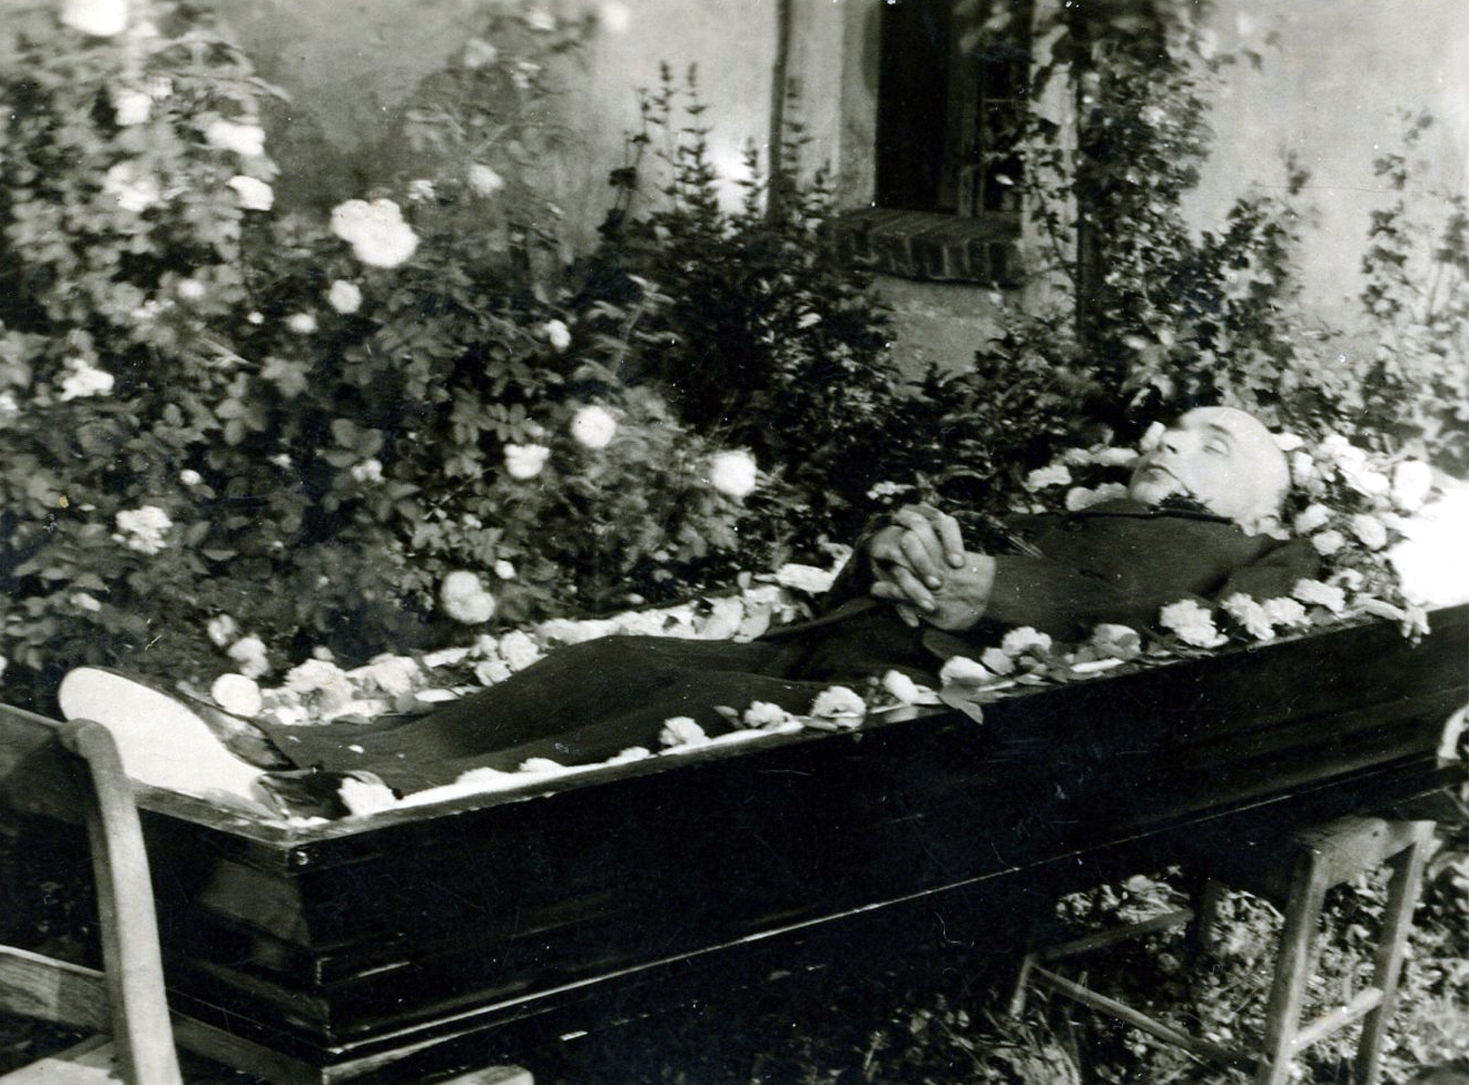
\includegraphics[width=0.7\textwidth]{photo/wiktor_swierczynski_pogrzeb.jpg}
\caption[Wiktor Świerczyński w trumnie]{Wiktor Świerczyński w trumnie - ofiara hitlerowskiego ludobójstwa.}
\label{rys:wiktor_swierczynski_pogrzeb}
\end{center}
\end{figure}

Czy tak musiało się stać? Dlaczego Opatrzność Boża dopuściła do tej zbrodni??? Po pierwsze trzeba by zapytać, gdzie stryjowi Wiktorowi byłoby lepiej: czy tu na ziemi leżeć sztywno i bezczynnie w łóżku, cierpliwie znosząc swoje kalectwo i pozostawanie na łaskawym chlebie, a był przecież człowiekiem ambitnym, czy też Tam, u bogatego w Miłosierdzie Boga?! Odpowiedź jest oczywista, że Bóg wybrał najlepsze rozwiązanie, gdyż stryj  Wiktor swymi niezawinionymi cierpieniami oraz swą aktywnością majsterkowicza zaskarbił sobie wdzięczność wielu ludzi, także dzieci rzeźbiąc im zabawki i fujarki do grania,\ldots a dopuścił Bóg do zbrodni, ,,aby okazały się zamysły serc wielu'' i okazały się! Tak działa Opatrzność Boża, zawsze genialnie i zawsze z miłością, nie czyniąc krzywdy, lecz karząc winowajców zbrodni i wynagradzając niewinnych maluczkich za ich cierpienia i miłosierdzie względem swych bliźnich, a takim właśnie był stryj Wiktor -- wielki duchem Człowiek.